\documentclass{article}
\usepackage{amsmath}
\usepackage{amsthm}
\usepackage{tikz}
\usetikzlibrary{arrows}
\newcommand\independent{\protect\mathpalette{\protect\independenT}{\perp}}
\def\independenT#1#2{\mathrel{\rlap{$#1#2$}\mkern2mu{#1#2}}}
\newtheorem{theorem}{Theorem}
\newtheorem{mydef}{Definition}
\title{Learning Neighborhoods: Method description part I -- The models}
\author{Forest Gregg}
\begin{document}
\maketitle
Say we would like to think how patterns of racial segregation in a
city could arise from individual choices of residents. We think there
is some process at the household level, that all else being equal,
makes it more likely that neighbors will be of the same race than
different races. We'd like to reason about what kinds of global patterns
of segregation are likely to arise from these local processes.

To get going, let's make a couple of simplifying assumptions. First,
we'll assume there are only two races: black and white. Second, we'll
assume that only direct neighbors affect whether a black or white
family lives in a house. More distant neighbors can influence the
house, but only by influencing a directly neighboring house.

From these assumptions, we can build a probability distribution over
all global patterns of racial segregation in a city, from complete
segregation to complete integration.


Let's look at four houses, that we will call $A$, $B$, $C$, and $D$,
Houses $A$ and $C$ are not neighbors and neither are $B$ and $D$ (figure X).

Now, let's say there is a particular pattern of black and white
houses, for example House A--black, House B--black, House C--white,
House D--white. We'll call this particular pattern $x$, and we'll say
that $\Pr(X=x)$ is the probability of that pattern, and $\Pr(X)$ is
the probability distribution over all possible patterns

We'd like to express this probability distribution only in terms of
local interactions between neighboring houses. We'll do this in two
steps. First we'll show that any probability distribution over these
four houses can be expressed as a product of functions that only take
in the value of neighboring houses, i.e. :

\begin{equation}
  \Pr(X) = \phi_1(A,B)\phi_2(B,C)\phi_3(C,D)\phi_4(D,A) 
\end{equation}

Second, we'll choose functions that compactly express our assumptions
about local interactions.

\subsection*{Independence and Factorization}
Because we think that houses can only influence each other through a
direct neighbor, we can say that $A$ and $C$ are independent of each
other given their immediate neighbors $B$ and $D$, and that $B$ and
$D$ are independent given $A$ and $C$. This does not mean that $A$ can
not influence $C$ just that the influence must operate through $B$ and
$D$. If we already know $B$ and $D$, then we have fully taken into
account the influence of $A$ on $C$.

As I'll demonstrate these independencies imply that

\begin{equation}
\Pr(X) = \phi_1(A,B)\phi_2(B,C)\phi_3(C,D)\phi_4(D,A) 
\end{equation}


\subsection*{Factorization}

\begin{theorem}
Let $A$, $B$, and $C$ be three disjoint sets of variables such that
$X = A \cup B \cup C$. $\Pr(X)$ satisfies $(A\independent B) \mid C$
if and only if


\begin{equation}
\Pr(X) = \phi_1(A,C)\phi_2(B,C)
\end{equation}

for some functions $\phi_1$ and $\phi_2$.
\end{theorem}

\begin{proof}
Assume that $(A\independent B) \mid C$
\begin{align}
\Pr(A,B,C) &= \Pr(A,B \mid C)\Pr(C) \\
&= \Pr(A \mid C)\Pr(B \mid C)\Pr(C) \\
&= \phi_1(A,C)\phi_2(B,C)
\end{align}

Where we set $\phi_1(A,C) = \Pr(A \mid C)$ and $\phi_2 = \Pr(B \mid
C)\Pr(C)$. \\

Now assume that $\Pr(A,B,C) = \phi_2(A,C)\phi_2(B,C)$. Let
$\phi_3(C)=\sum_A\phi_1(A,C)$ and $\phi_4(C)=\sum_B\phi_2(B,C)$.

\begin{align}
\Pr(A,B \mid C) &= \frac{\Pr(A,B,C)}{\sum_{A,B}\Pr(A,B,C)} \\
&= \frac{\phi_1(A,C)\phi_2(B,C)}{\sum_{A,B}\phi_2(A,C)\phi_2(B,C)} \\
&= \frac{\phi_1(A,C)\phi_2(B,C)}{\phi_3(C)\phi_4(C)}
\end{align}

Similarly

\begin{align}
\Pr(A \mid C) &= \frac{\sum_B\Pr(A,B,C)}{\sum_{A,B}\Pr(A,B,C)} \\
&= \frac{\phi_1(A,C)\phi_4(C)}{\phi_3(C)\phi_4(C)} \\
&= \frac{\phi_1(A,C)}{\phi_3(C)}
\end{align}

From which we can see that 

\begin{equation}
\Pr(A,B \mid C) = \Pr(A \mid C)\Pr(B \mid C)
\end{equation}

Which was to be proven.
\end{proof}

Now, if we let $\phi_5(A,B,D) = \phi_1(A,B)\phi_4(D,A)$ and $\phi_6(C,B,D) = \phi_2(B,C)\phi_3(C,D)$ we can see that 

\begin{align}
\Pr(X) &= \phi_1(A,B)\phi_2(B,C)\phi_3(C,D)\phi_4(D,A) \\
&= \phi_5(A,B,D)\phi_6(C,B,D) \\
&= \phi_5(A,\left\{B,D\right\})\phi_6(C,\left\{B,D\right\})
\end{align}

which implies $(A\independent C) \mid (B,D)$, and if we combine the factors 
another way it also implies $(B\independent D) \mid (A,C)$.

\section{Factors to Distributions}
We have see that there is an intimate connection between the
independencies respected by a probability distribution and the
factorization of that distribution into functions. In particular, we
have shown that a probability distribution with certain independencies
can be factored into functions that have only directly dependent
random variables in their scope.

Remember that we represented the dependencies between the houses as
edges. We drew an edge between two houses when the houses had a
direct, unmediated effect upon each other. Networks of this kind are
called Markov networks, and what we saw for our example is true for
all networks of this type.

\begin{mydef}
A distribution $\Pr_{\phi}$ is a Gibbs distribution defined by the factors
$\left\{\phi_1(D_1),...,\phi_K(D_k)\right\}$ if

\begin{equation}
\Pr_{\phi}(X_1,...X_n) = \frac{1}{Z}\tilde{P_{\phi}}(X_1,...,X_n)
\end{equation}

where
\begin{equation}
\tilde{P_{\phi}}(X_1,...,X_n) = \phi_1(D_1)\phi_2(D_2)...\phi_{K-1}(D_{K-1})\phi_K(D_k)
\end{equation}

and

\begin{equation}
Z = \sum_{X_1,...,X_n}\tilde{P_{\phi}}(X_1,...,X_n)
\end{equation}
\end{mydef}

A Gibbs distribution is the probability distribution with maximum
entropy given some constraint. For example, the uniform distribution
is the maximum entropy distribution that has support on a given
interval $[a,b]$, the exponential distribution is the maximum entropy
distribution given a positive mean, and the normal distribution is the
maximum entropy distribution given a mean and a standard
deviation. The $\phi$'s can be thought of as Lagrangian encoding of
constraints.

\begin{mydef}
A distribution
$P(X)=\frac{1}{Z}\phi_1(D_1)\phi_2(D_2)...\phi_{K-1}(D_{K-1})\phi_K(D_k)$
factorizes over a Markov network $H$ if each $D_k$ is a complete
subgraph of $H$.
\end{mydef}

 As a reminder a complete subgraph is set of nodes in
a network where there is a direct connection between all of the nodes,
also called a clique.

\begin{mydef}
Let $H$ be a Markov network structure, and let $X_1--...--X_k$ be a
path in $H$. Let $Z \in X$ be a set of observed variables. The path
$X_1-...-X_k$ is active given $Z$ if none of the $X_i$'s, $i =
1,...k$ is in $Z$.
\end{mydef}

\begin{mydef}
A set of nodes $Z$ separates $X$ and $Y$ in $H$, which we denote
$\operatorname{sep}_H(X;Y \mid Z)$ if there is no active path between
nodes $X \in X$ and $Y \in Y$ given $Z$. We define the global
independencies associated with $H$ to be $I(H) = \left\{(X \independent Y \mid Z) : \operatorname{sep}_H(X;Y \mid Z)\right\}$.
\end{mydef}

From a proof similar to the one above and the Hammersly-Clifford
theorem, it turns out that the following theorems hold

\begin{theorem}
  If P is a Gibbs distribution, then P factorizes over a Markov network
H if and only if every independency in P is encoded in H
\end{theorem}

\section{Parameterization}
Returning to our four house example, we saw that we can express the
probability of the pattern of an assignment to all the houses can be
factored into functions that only look at the interactions between
neighboring houses. But we still need to choose the form of the
functions $\phi$.

\begin{equation}
\Pr(X) = \phi_1(A,B)\phi_2(B,C)\phi_3(C,D)\phi_4(D,A) 
\end{equation}


 
To return to our original assumptions, we said that we think that a
black house has some influence on neighboring houses to make them
black. Let's call that influence $w$. And we'll assume that white
houses have the same influence, but in the opposite direction,
i.e. $-w$.\footnote{I believe, but have not proven that this
  assumption of 'symmetry of influence' is required if we want
  represent the system as a Markov field.}


For a particular house $i$, the balance of influence $h_I$ depends upon the
number of white neighboring houses, $n_W$ and black neighboring houses $n_B$.

\begin{equation}
h_i = w(n_W - n_B)
\end{equation}

and we'll say that the probability the race of a house is

\begin{align}
\Pr(\text{house}_i = \text{white}) = \frac{e^{h_i}}{e^{h_i} + e^{-h_i}} \\
\Pr(\text{house}_i = \text{black}) = \frac{e^{-h_i}}{e^{h_i} + e^{-h_i}} \\
\end{align}

And that the probability for any particular pattern of race is

\begin{equation}
\Pr(X) = \prod\frac{e^{R_ih_i}}{e^{h_i} + e^{-h_i}}
\end{equation}

Where $R_i$ is an indicator variable that takes a value of
$1$ where the race of the house is white and a value of $-1$ if the
house is black.

We can also express this probability in terms of the pairwise interactions 
of neighbors.

\begin{align}
\Pr(X) &= \prod_i\frac{e^{R_ih_i}}{e^{h_i} + e^{-h_i}} \\
&= \prod_i\frac{\prod_{j \in <i j>}e^{R_iR_jw}}{e^{h_i} + e^{-h_i}} \\
\end{align}

Where $j \in <i j>$ are all the sites that are nearest neighbors of site $i$. Each pair will be appear in the numerator twice. So that 

\begin{align}
\Pr(X) &= \frac{1}{Z}\prod_{<i j>'}e^{R_iR_jw'} \\
&= \frac{1}{Z}\operatorname{exp}(\sum_{<i j>'}R_iR_jw') 
\end{align}

Where $Z$ is normalizing constant that is the sum of all possible assignments, 
$<i j>'$ is every nearest neighbor only counted once, and $w' = w/2$.

We can see that it is a Gibbs distribution and we can also see that it
encodes the same independencies of our racial preference house model,
so that this distribution factorizes over our network of influence.

\section{Extensions}
While we have shown how we can develop an relatively simple formula
for the probability distribution over global patterns that arise from
local interactions. In the model we worked through, the smallest unit
is only influenced by it's immediate neighbors and can only take on
two values--either the house is occupied by a black family or a white
one. 

Perhaps we think that there are some other differences among houses
that make it more likely for one race to occupy it than another.
We can naturally extend the model to include a house specific term $u_i$.

\begin{align}
\Pr(X) &= \frac{1}{Z}\operatorname{exp}(\sum_{<i j>'}R_iR_jw' + \sum_iu_iR_i) 
\end{align}

Indeed, we are not limited to multiplication, but can use choose any
functions $\epsilon_{i,j}$ and $\epsilon_i$, and we will still have a valid 
probability distribution over global patterns.

\begin{equation}
\Pr(X) = \frac{1}{Z}\operatorname{exp}(\sum_{<i j>'}\epsilon_{i,j}(R_i,R_j) + \sum_i\epsilon_i(R_i)) 
\end{equation}

A simple choice of $\epsilon_{i,j}$ that will allow us to deal with
more than two races is

\begin{equation}
\epsilon_{i,j}(R_i,R_j) = \begin{cases}
  0 \quad\quad R_i = R_j \\
  \lambda_{i,j} \quad R_i \neq R_j
\end{cases}
\end{equation}

Or the model can be extended so that $\epsilon_{i,j}$ is a
site specific distance function between $x_i$ and $x_j$ so that
likelihood of neighbors being the same race can be function of how
similar they are in other ways. 

\section{Neighborhoods}
The time has come to leave discussion of racial segregation, and take
up the phenomena we are really interested in here: neighborhoods.

If we make the assumption that a household can belong to one and only
one neighborhood, we can use all the machinery of Markov Random Fields
we just developed to try to learn what are the features, block by
block that cohere into a neighborhood. This is a very troublesome
assumption, and we we'll return to it , but let's see what we can do
if we make it.

We'll use this machinery twice. First, we'll use it to help create a
set of target ``neighborhoods'' and then we'll use it to learn what
local features might have produced those neighborhoods. But to explain
how we'll do that I need to explain how we go about getting real
values from these beautiful equations. As it turns out this is a pretty 
complicated question, which I'll take up in the next dispatch.






\end{document}
The log probability can be expressed a good deal more simply. 


 







two neighboring houses are both white or both black, then


\begin{figure}
\centering
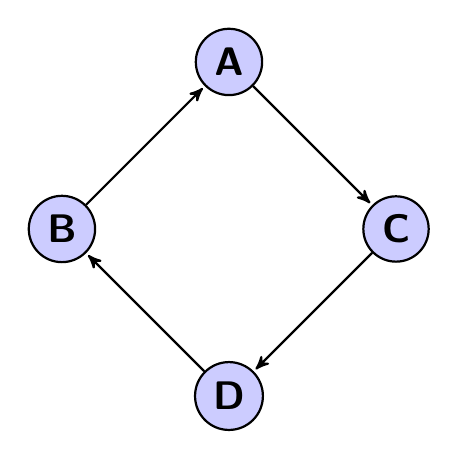
\begin{tikzpicture}[->,>=stealth',shorten >=1pt,auto,node distance=3cm,
  thick,main node/.style={circle,fill=blue!20,draw,font=\sffamily\Large\bfseries}]

  \node[main node] (1) {A};
  \node[main node] (2) [below left of=1] {B};
  \node[main node] (3) [below right of=2] {D};
  \node[main node] (4) [below right of=1] {C};

  \path[every node/.style={font=\sffamily\small}]
    (1) edge node [left] {} (4)
    (2) edge node [right] {} (1)
    (3) edge node [right] {} (2)
    (4) edge node [left] {} (3);
\end{tikzpicture}
\caption{Markovian Dependent Variables}
\end{figure}



 be random variables, and let $X$ be the
joint assignment of these four variables.



 that take
on the values 1 or 0.



These variables can take on $2^4$ permutations. In general, if we are
interested in the probability of any these permutations we need to
keep track of sixteen separate values.

\begin{align*}
&\Pr(A=0,B=0,C=0,D=0) = P_1 \\
&\Pr(A=1,B=0,C=0,D=0) = P_2 \\
&\Pr(A=0,B=1,C=0,D=0) = P_3 \\
&\vdots \\
&\Pr(A=1,B=1,C=0,D=1) = P_{14} \\
&\Pr(A=1,B=1,C=1,D=0) = P_{15} \\
&\Pr(A=1,B=1,C=1,D=1) = P_{16} 
\end{align*}

However, if these variables are independent, then we only need to know
four values -- the probability of each random variable taking a value.

Independence means that the probability of realizing a permutation of
values factors into the product of each value taking on the
corresponding value.

\begin{equation}
\Pr(A,B,C,D) = \Pr(A)\Pr(B)\Pr(C)\Pr(D)
\end{equation}

\section*{Representing Dependence}

We can represent the dependence and independence relations between random
variables in a graph. If the four variables are independent, then we draw
the variables as nodes with no edges between them.


\begin{figure}[!ht]
\centering
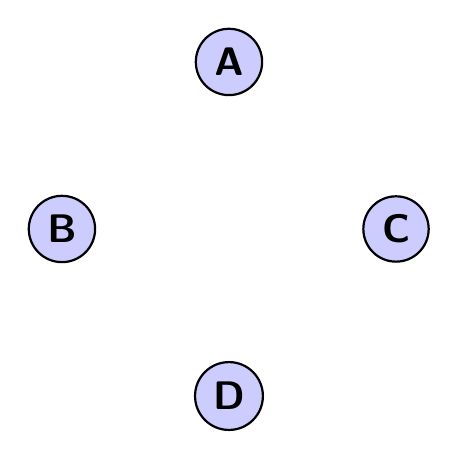
\begin{tikzpicture}[->,>=stealth',shorten >=1pt,auto,node distance=3cm,
  thick,main node/.style={circle,fill=blue!20,draw,font=\sffamily\Large\bfseries}]

  \node[main node] (1) {A};
  \node[main node] (2) [below left of=1] {B};
  \node[main node] (3) [below right of=2] {D};
  \node[main node] (4) [below right of=1] {C};


\end{tikzpicture}
\caption{Completely Independent Variables}
\end{figure}

On the other hand, if each variable is dependent on all the others,
then the graph is completely connected. 

\begin{figure}
\centering
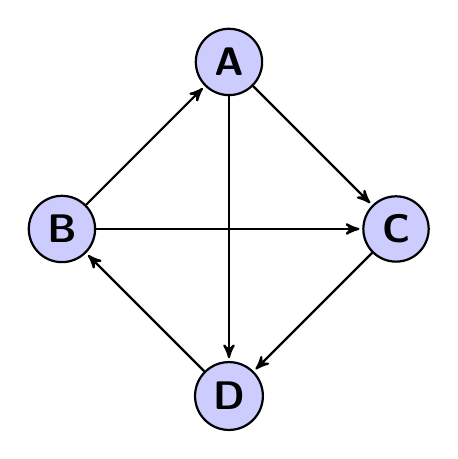
\begin{tikzpicture}[->,>=stealth',shorten >=1pt,auto,node distance=3cm,
  thick,main node/.style={circle,fill=blue!20,draw,font=\sffamily\Large\bfseries}]

  \node[main node] (1) {A};
  \node[main node] (2) [below left of=1] {B};
  \node[main node] (3) [below right of=2] {D};
  \node[main node] (4) [below right of=1] {C};

  \path[every node/.style={font=\sffamily\small}]
    (1) edge node [left] {} (4)
        edge node [left] {} (3)
    (2) edge node [right] {} (1)
        edge node {} (4)
    (3) edge node [right] {} (2)
    (4) edge node [left] {} (3);
\end{tikzpicture}
\caption{Completely Dependent Variables}
\end{figure}

Now, let's consider an intermediate graph. In this graph, conditional
on its neighbors, a random value is independent of all other values. 

\begin{figure}
\centering
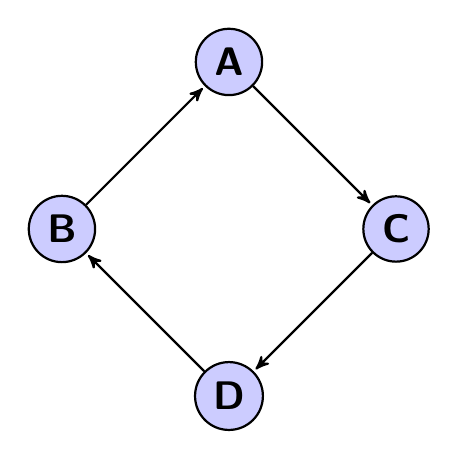
\begin{tikzpicture}[->,>=stealth',shorten >=1pt,auto,node distance=3cm,
  thick,main node/.style={circle,fill=blue!20,draw,font=\sffamily\Large\bfseries}]

  \node[main node] (1) {A};
  \node[main node] (2) [below left of=1] {B};
  \node[main node] (3) [below right of=2] {D};
  \node[main node] (4) [below right of=1] {C};

  \path[every node/.style={font=\sffamily\small}]
    (1) edge node [left] {} (4)
    (2) edge node [right] {} (1)
    (3) edge node [right] {} (2)
    (4) edge node [left] {} (3);
\end{tikzpicture}
\caption{Markovian Dependent Variables}
\end{figure}

Unlike the first case. $A\not\independent D$ and $B\not\independent
C$, but $(A\independent D) \mid (B,C)$, and $(B\independent C) \mid
(A,D)$.

\end{document}

Let's set up some definitions.

A distribution $\Pr_{\phi}$ is a Gibbs distribution defined by the factors
$\left\{\phi_1(D_1),...,\phi_K(D_k)\right\}$ if

\begin{equation}
\Pr_{\phi}(X_1,...X_n) = \frac{1}{Z}\tilde{P_{\phi}}(X_1,...,X_n)
\end{equation}

where
\begin{equation}
\tilde{P_{\phi}}(X_1,...,X_n) = \phi_1(D_1)\phi_2(D_2)...\phi_{K-1}(D_{K-1})\phi_K(D_k)
\end{equation}

and

\begin{equation}
Z = \sum_{X_1,...,X_n}\tilde{P_{\phi}}(X_1,...,X_n)
\end{equation}


We say that a distribution
$P(X)=\frac{1}{Z}\phi_1(D_1)\phi_2(D_2)...\phi_{K-1}(D_{K-1})\phi_K(D_k)$
factorizes over a Markov network $H$ if each $D_k$ is a complete
subgraph of $H$.

Let $H$ be a Markov network structure, and let $X_1--...--X_k$ be a
path in $H$. Let $Z \in X$ be a set of observed variables. The path
$X_1--...--X_k$ is active given $Z$ if none of the $X_i$'s, $i =
1,...k$ is in $Z$.



A set of nodes $Z$ separates $X$ and $Y$ in $H$, which we denote
$\operatorname{sep}_H(X;Y \mid Z)$ if there is no active path between
nodes $X \in X$ and $Y \in Y$ given $Z$. We define the global
independencies associated with $H$ to be


I won't got proof now, but just emphasize the key point. Every Markov
network represents 

positive distribution P factorizes over a
Markov network $H$ if and only if $H$ encodes every independency in P.

This means that 




It turns out that was true for our simple example is true for a whole
class of networks called Markov Networks.




We represented our four random variables as a network, where two variables
shared an edge if and only if two variables were directly dependent. This graph is an instance of a class of graphs 


It turns out that what was true for our simple example is true for all
Markov networks. 

Some definitions



We can go further 
and say that 

we have seen that we can factor 


Where $phi$ is special kind of function called a factor, which has the
property that 

These independencies allow us to begin 



